% This is "sig-alternate.tex" V1.8 June 2007 Modified for SOUPS 2014
% This file should be compiled with V2.3 of "sig-alternate.cls" June 2007
%
% This example file demonstrates the use of the 'sig-alternate.cls'
% V2.3 LaTeX2e document class file. It is for those submitting
% articles to ACM Conference Proceedings WHO DO NOT WISH TO
% STRICTLY ADHERE TO THE SIGS (PUBS-BOARD-ENDORSED) STYLE.
% The 'sig-alternate.cls' file will produce a similar-looking,
% albeit, 'tighter' paper resulting in, invariably, fewer pages.
%
% ----------------------------------------------------------------------------------------------------------------
% This .tex file (and associated .cls V2.3) produces:
%       1) The Permission Statement
%       2) The Conference (location) Info information
%       3) The Copyright Line with ACM data
%       4) NO page numbers
%
% as against the acm_proc_article-sp.cls file which
% DOES NOT produce 1) thru' 3) above.
%
% Using 'sig-alternate.cls' you have control, however, from within
% the source .tex file, over both the CopyrightYear
% (defaulted to 200X) and the ACM Copyright Data
% (defaulted to X-XXXXX-XX-X/XX/XX).
% e.g.
% \CopyrightYear{2007} will cause 2007 to appear in the copyright line.
% \crdata{0-12345-67-8/90/12} will cause 0-12345-67-8/90/12 to appear in the copyright line.
%
% ---------------------------------------------------------------------------------------------------------------
% This .tex source is an example which *does* use
% the .bib file (from which the .bbl file % is produced).
% REMEMBER HOWEVER: After having produced the .bbl file,
% and prior to final submission, you *NEED* to 'insert'
% your .bbl file into your source .tex file so as to provide
% ONE 'self-contained' source file.
%
% ================= IF YOU HAVE QUESTIONS =======================
% Questions regarding the SIGS styles, SIGS policies and
% procedures, Conferences etc. should be sent to
% Adrienne Griscti (griscti@acm.org)
%
% Technical questions _only_ to
% Gerald Murray (murray@acm.org)
% ===============================================================
%
% For tracking purposes - this is V1.8 - June 2007

% --- Start page size ---
%Please use the following format  
\documentclass[twoside,letterpaper]{soups} 
\pdfpagewidth=8.5truein 
\pdfpageheight=11truein 
% --- End page size ---


\usepackage{graphicx}
\usepackage{times}
\renewcommand{\topfraction}{0.99} % be more aggressive about text around floats
\renewcommand{\floatpagefraction}{0.99}
\pagestyle{plain} % page numbers

\begin{document}
%
% --- Author Metadata here ---
\conferenceinfo{Symposium on Usable Privacy and Security
  (SOUPS)}{2016, June 22--24, 2016, Denver, Colorado.}
\CopyrightYear{2016} % Allows default copyright year (200X) to be over-ridden - IF NEED BE.
%\crdata{0-12345-67-8/90/01}  % Allows default copyright data (0-89791-88-6/97/05) to be over-ridden - IF NEED BE.
% --- End of Author Metadata ---

\title{Our Workshop Paper in the SOUPS 2016 Template. Please look at the aside, methodology, and results%
\titlenote{(Produces the permission block, and copyright information). For use with SIG-ALTERNATE.CLS. Supported by ACM.}}
\subtitle{Subtitle (optional)%
\titlenote{A full version of this paper is available as
\textit{Author's Guide to Preparing ACM SIG Proceedings Using
\LaTeX$2_\epsilon$\ and BibTeX} at
\texttt{www.acm.org/sigs/publications/sigguide-v2.2sp}}}
%
% You need the command \numberofauthors to handle the 'placement
% and alignment' of the authors beneath the title.
%
% For aesthetic reasons, we recommend 'three authors at a time'
% i.e. three 'name/affiliation blocks' be placed beneath the title.
%
% NOTE: You are NOT restricted in how many 'rows' of
% "name/affiliations" may appear. We just ask that you restrict
% the number of 'columns' to three.
%
% Because of the available 'opening page real-estate'
% we ask you to refrain from putting more than six authors
% (two rows with three columns) beneath the article title.
% More than six makes the first-page appear very cluttered indeed.
%
% Use the \alignauthor commands to handle the names
% and affiliations for an 'aesthetic maximum' of six authors.
% Add names, affiliations, addresses for
% the seventh etc. author(s) as the argument for the
% \additionalauthors command.
% These 'additional authors' will be output/set for you
% without further effort on your part as the last section in
% the body of your article BEFORE References or any Appendices.

\numberofauthors{8} %  in this sample file, there are a *total*
% of EIGHT authors. SIX appear on the 'first-page' (for formatting
% reasons) and the remaining two appear in the \additionalauthors section.
%
\author{
% You can go ahead and credit any number of authors here,
% e.g. one 'row of three' or two rows (consisting of one row of three
% and a second row of one, two or three).
%
% The command \alignauthor (no curly braces needed) should
% precede each author name, affiliation/snail-mail address and
% e-mail address. Additionally, tag each line of
% affiliation/address with \affaddr, and tag the
% e-mail address with \email.
%
% 1st. author
\alignauthor
Tyler W Thomas\titlenote{author 1 note here.}\\
       \affaddr{Institute for Clarity in Documentation}\\
       \affaddr{1932 Wallamaloo Lane}\\
       \affaddr{Wallamaloo, New Zealand}\\
       \email{trovato@corporation.com}
% 2nd. author
\alignauthor
Justin Smith\titlenote{author 2 note here}\\
       \affaddr{Institute for Clarity in Documentation}\\
       \affaddr{P.O. Box 1212}\\
       \affaddr{Dublin, Ohio 43017-6221}\\
       \email{webmaster@marysville-ohio.com}
% 3rd. author
\alignauthor Heather Lipford{\o}rv{\"a}ld\titlenote{author 3 note here}\\
       \affaddr{The Th{\o}rv{\"a}ld Group}\\
       \affaddr{1 Th{\o}rv{\"a}ld Circle}\\
       \affaddr{Hekla, Iceland}\\
       \email{larst@affiliation.org}
\and  % use '\and' if you need 'another row' of author names
% 4th. author
\alignauthor Bill Chu\\
       \affaddr{Brookhaven Laboratories}\\
       \affaddr{Brookhaven National Lab}\\
       \affaddr{P.O. Box 5000}\\
       \email{lleipuner@researchlabs.org}
% 5th. author
\alignauthor Emerson Murphy-Hill\\
       \affaddr{NASA Ames Research Center}\\
       \affaddr{Moffett Field}\\
       \affaddr{California 94035}\\
       \email{fogartys@amesres.org}
}
% There's nothing stopping you putting the seventh, eighth, etc.
% author on the opening page (as the 'third row') but we ask,
% for aesthetic reasons that you place these 'additional authors'
% in the \additional authors block, viz.
\additionalauthors{Additional authors: John Smith (The Th{\o}rv{\"a}ld Group,
email: {\texttt{jsmith@affiliation.org}}) and Julius P.~Kumquat
(The Kumquat Consortium, email: {\texttt{jpkumquat@consortium.net}}).}
\date{30 July 1999}
% Just remember to make sure that the TOTAL number of authors
% is the number that will appear on the first page PLUS the
% number that will appear in the \additionalauthors section.

\maketitle
\begin{abstract}
This paper provides a sample of a \LaTeX\ document which conforms,
somewhat loosely, to the formatting guidelines for
ACM SIG Proceedings. It is an {\em alternate} style which produces
a {\em tighter-looking} paper and was designed in response to
concerns expressed, by authors, over page-budgets.
It complements the document \textit{Author's (Alternate) Guide to
Preparing ACM SIG Proceedings Using \LaTeX$2_\epsilon$\ and Bib\TeX}.
This source file has been written with the intention of being
compiled under \LaTeX$2_\epsilon$\ and BibTeX.

The developers have tried to include every imaginable sort
of ``bells and whistles," such as a subtitle, footnotes on
title, subtitle and authors, as well as in the text, and
every optional component (e.g. Acknowledgments, Additional
Authors, Appendices), not to mention examples of
equations, theorems, tables and figures.

To make best use of this sample document, run it through \LaTeX\
and BibTeX, and compare this source code with the printed
output produced by the dvi file. A compiled PDF version
is available on the web page to help you with the
`look and feel'.
\end{abstract}


\section{Introduction}
The \textit{proceedings} are the records of a conference.
SOUPS hopes to give these conference by-products a uniform,
high-quality appearance.  To do this, there are some rigid
requirements for the format of the proceedings documents: there
is a specified format (balanced  double columns), a specified
set of fonts (Arial or Helvetica and Times Roman) in
certain specified sizes (for instance, 9 point for body copy),
a specified live area (18 $\times$ 23.5 cm [7" $\times$ 9.25"]) centered on
the page, specified size of margins (2.54cm [1"] top and
bottom and 1.9cm [.75"] left and right; specified column width
(8.45cm [3.33"]) and gutter size (.083cm [.33"]).

The good news is, with only a handful of manual
settings\footnote{Two of these, the {\texttt{\char'134 numberofauthors}}
and {\texttt{\char'134 alignauthor}} commands, you have
already used; another, {\texttt{\char'134 balancecolumns}}, will
be used in your very last run of \LaTeX\ to ensure
balanced column heights on the last page.}, the \LaTeX\ document
class file handles all of this for you.

The remainder of this document is concerned with showing, in
the context of an ``actual'' document, the \LaTeX\ commands
specifically available for denoting the structure of a
proceedings paper, rather than with giving rigorous descriptions
or explanations of such commands.

\section{The {\secit Body} of The Paper}
Typically, the body of a paper is organized
into a hierarchical structure, with numbered or unnumbered
headings for sections, subsections, sub-subsections, and so on. 
The command \texttt{{\char'134}section} that
precedes this paragraph is part of such a
hierarchy.\footnote{This is the second footnote.  It
starts a series of three footnotes that add nothing
informational, but just give an idea of how footnotes work
and look. It is a wordy one, just so you see
how a longish one plays out.} \LaTeX\ handles the numbering
and placement of these headings for you, when you use
the appropriate heading commands around the titles
of the headings.  If you want a sub-subsection or
smaller part to be unnumbered in your output, simply append an
asterisk to the command name.  Examples of both
numbered and unnumbered headings will appear throughout the
balance of this sample document.

Because the entire article is contained in
the \textbf{document} environment, you can indicate the
start of a new paragraph with a blank line in your
input file; that is why this sentence forms a separate paragraph.

\subsection{Type Changes and {\subsecit Special} Characters}
We have already seen several typeface changes in this sample.  You
can indicate italicized words or phrases in your text with
the command \texttt{{\char'134}textit}; emboldening with the
command \texttt{{\char'134}textbf}
and typewriter-style (for instance, for computer code) with
\texttt{{\char'134}texttt}.  But remember, you do not
have to indicate typestyle changes when such changes are
part of the \textit{structural} elements of your
article; for instance, the heading of this subsection will
be in a sans serif\footnote{A third footnote, here.
Let's make this a rather short one to
see how it looks.} typeface, but that is handled by the
document class file. Take care with the use
of\footnote{A fourth, and last, footnote.}
the curly braces in typeface changes; they mark
the beginning and end of
the text that is to be in the different typeface.

You can use whatever symbols, accented characters, or
non-English characters you need anywhere in your document;
you can find a complete list of what is
available in the \textit{\LaTeX\
User's Guide} \cite{Lamport:LaTeX}.

\subsection{Math Equations}
You may want to display math equations in three distinct styles:
inline, numbered, or non-numbered display.  Each of
the three are discussed in the next sections.

\subsubsection{Inline (In-text) Equations}
A formula that appears in the running text is called an
inline or in-text formula.  It is produced by the
\textbf{math} environment, which can be
invoked with the usual \texttt{{\char'134}begin. . .{\char'134}end}
construction or with the short form \texttt{\$. . .\$}. You
can use any of the symbols and structures,
from $\alpha$ to $\omega$, available in
\LaTeX\cite{Lamport:LaTeX}; this section will simply show a
few examples of in-text equations in context. Notice how
this equation: \begin{math}\lim_{n\rightarrow \infty}x=0\end{math},
set here in in-line math style, looks slightly different when
set in display style.  (See next section).

\subsubsection{Display Equations}
A numbered display equation -- one set off by vertical space
from the text and centered horizontally -- is produced
by the \textbf{equation} environment. An unnumbered display
equation is produced by the \textbf{displaymath} environment.

Again, in either environment, you can use any of the symbols
and structures available in \LaTeX; this section will just
give a couple of examples of display equations in context.
First, consider the equation, shown as an inline equation above:
\begin{equation}\lim_{n\rightarrow \infty}x=0\end{equation}
Notice how it is formatted somewhat differently in
the \textbf{displaymath}
environment.  Now, we'll enter an unnumbered equation:
\begin{displaymath}\sum_{i=0}^{\infty} x + 1\end{displaymath}
and follow it with another numbered equation:
\begin{equation}\sum_{i=0}^{\infty}x_i=\int_{0}^{\pi+2} f\end{equation}
just to demonstrate \LaTeX's able handling of numbering.

\subsection{Citations}
Citations to articles \cite{bowman:reasoning,
braams:babel, clark:pct, herlihy:methodology},
conference proceedings \cite{clark:pct} or
books \cite{Lamport:LaTeX, salas:calculus} listed
in the Bibliography (or ``References'') section of your
article will occur throughout the text of your article.
You should use BibTeX to automatically produce this bibliography;
you simply need to insert one of several citation commands with
a key of the item cited in the proper location in
the \texttt{.tex} file \cite{Lamport:LaTeX}.
The key is a short reference you invent to uniquely
identify each work; in this sample document, the key is
the first author's surname and a
word from the title.  This identifying key is included
with each item in the \texttt{.bib} file for your article.

The details of the construction of the \texttt{.bib} file
are beyond the scope of this sample document, but more
information can be found in the \textit{Author's Guide},
and exhaustive details in the \textit{\LaTeX\ User's
Guide}\cite{Lamport:LaTeX}.

This article shows only the plainest form
of the citation command, using \texttt{{\char'134}cite}.
This is what is stipulated in the SIGS style specifications.
No other citation format is endorsed or supported.

Your reference list should be ordered alphabetically. When
citing more than one reference in the same set of brackets,
list the papers in ascending numerical order e.g., [1,2,3].

\subsection{Tables}
Because tables cannot be split across pages, the best
placement for them is typically the top of the page
nearest their initial cite.  To
ensure this proper ``floating'' placement of tables, use the
environment \textbf{table} to enclose the table's contents and
the table caption.  The contents of the table itself must go
in the \textbf{tabular} environment, to
be aligned properly in rows and columns, with the desired
horizontal and vertical rules.  Again, detailed instructions
on \textbf{tabular} material
is found in the \textit{\LaTeX\ User's Guide}.

Immediately following this sentence is the point at which
Table 1 is included in the input file; compare the
placement of the table here with the table in the printed
dvi output of this document.

\begin{table}
\centering
\caption{Frequency of Special Characters.}
\begin{tabular}{|c|c|l|} \hline
Non-English or Math&Frequency&Comments\\ \hline
\O & 1 in 1,000& For Swedish names\\ \hline
$\pi$ & 1 in 5& Common in math\\ \hline
\$ & 4 in 5 & Used in business\\ \hline
$\Psi^2_1$ & 1 in 40,000& Unexplained usage\\
\hline\end{tabular}
\end{table}

To set a wider table, which takes up the whole width of
the page's live area, use the environment
\textbf{table*} to enclose the table's contents and
the table caption.  As with a single-column table, this wide
table will ``float" to a location deemed more desirable.
Immediately following this sentence is the point at which
Table 2 is included in the input file; again, it is
instructive to compare the placement of the
table here with the table in the printed dvi
output of this document.


\begin{table*}
\centering
\caption{Some Typical Commands}
\begin{tabular}{|c|c|l|} \hline
Command&A Number&Comments\\ \hline
\texttt{{\char'134}alignauthor} & 100& Author alignment\\ \hline
\texttt{{\char'134}numberofauthors}& 200& Author enumeration\\ \hline
\texttt{{\char'134}table}& 300 & For tables\\ \hline
\texttt{{\char'134}table*}& 400& For wider tables\\ \hline\end{tabular}
\end{table*}
% end the environment with {table*}, NOTE not {table}!

\subsection{Figures}
Like tables, figures cannot be split across pages; the
best placement for them
is typically the top or the bottom of the page nearest
their initial cite.  To ensure this proper ``floating'' placement
of figures, use the environment
\textbf{figure} to enclose the figure and its caption.

This sample document contains examples of \textbf{.pdf}
files to be displayable with \LaTeX.  More
details on each of these is found in the \textit{Author's Guide}.

\begin{figure}
\centering

\includegraphics{fly}
\caption{A sample black and white graphic (.pdf format).}
\end{figure}

\begin{figure}
\centering

\includegraphics[height=1in,width=1in]{fly}
\caption{A sample black and white graphic (.pdf format)
that has been resized with the \texttt{includegraphics} command.}
\end{figure}


As was the case with tables, you may want a figure
that spans two columns.  To do this, and still to
ensure proper ``floating'' placement of tables, use the environment
\textbf{figure*} to enclose the figure and its caption.
\begin{figure*}
\centering
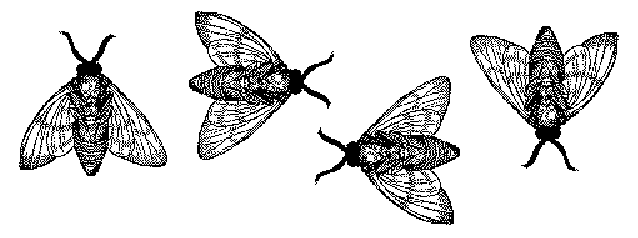
\includegraphics{flies}
\caption{A sample black and white graphic (.pdf format)
that spans two columns of text.}
\end{figure*}
and don't forget to end the environment with
{figure*}, not {figure}!

Note that either {\textbf{.pdf}} or {\textbf{.jpeg}} formats can be
included with the \verb+\includegraphics+ command.

\begin{figure}
\centering
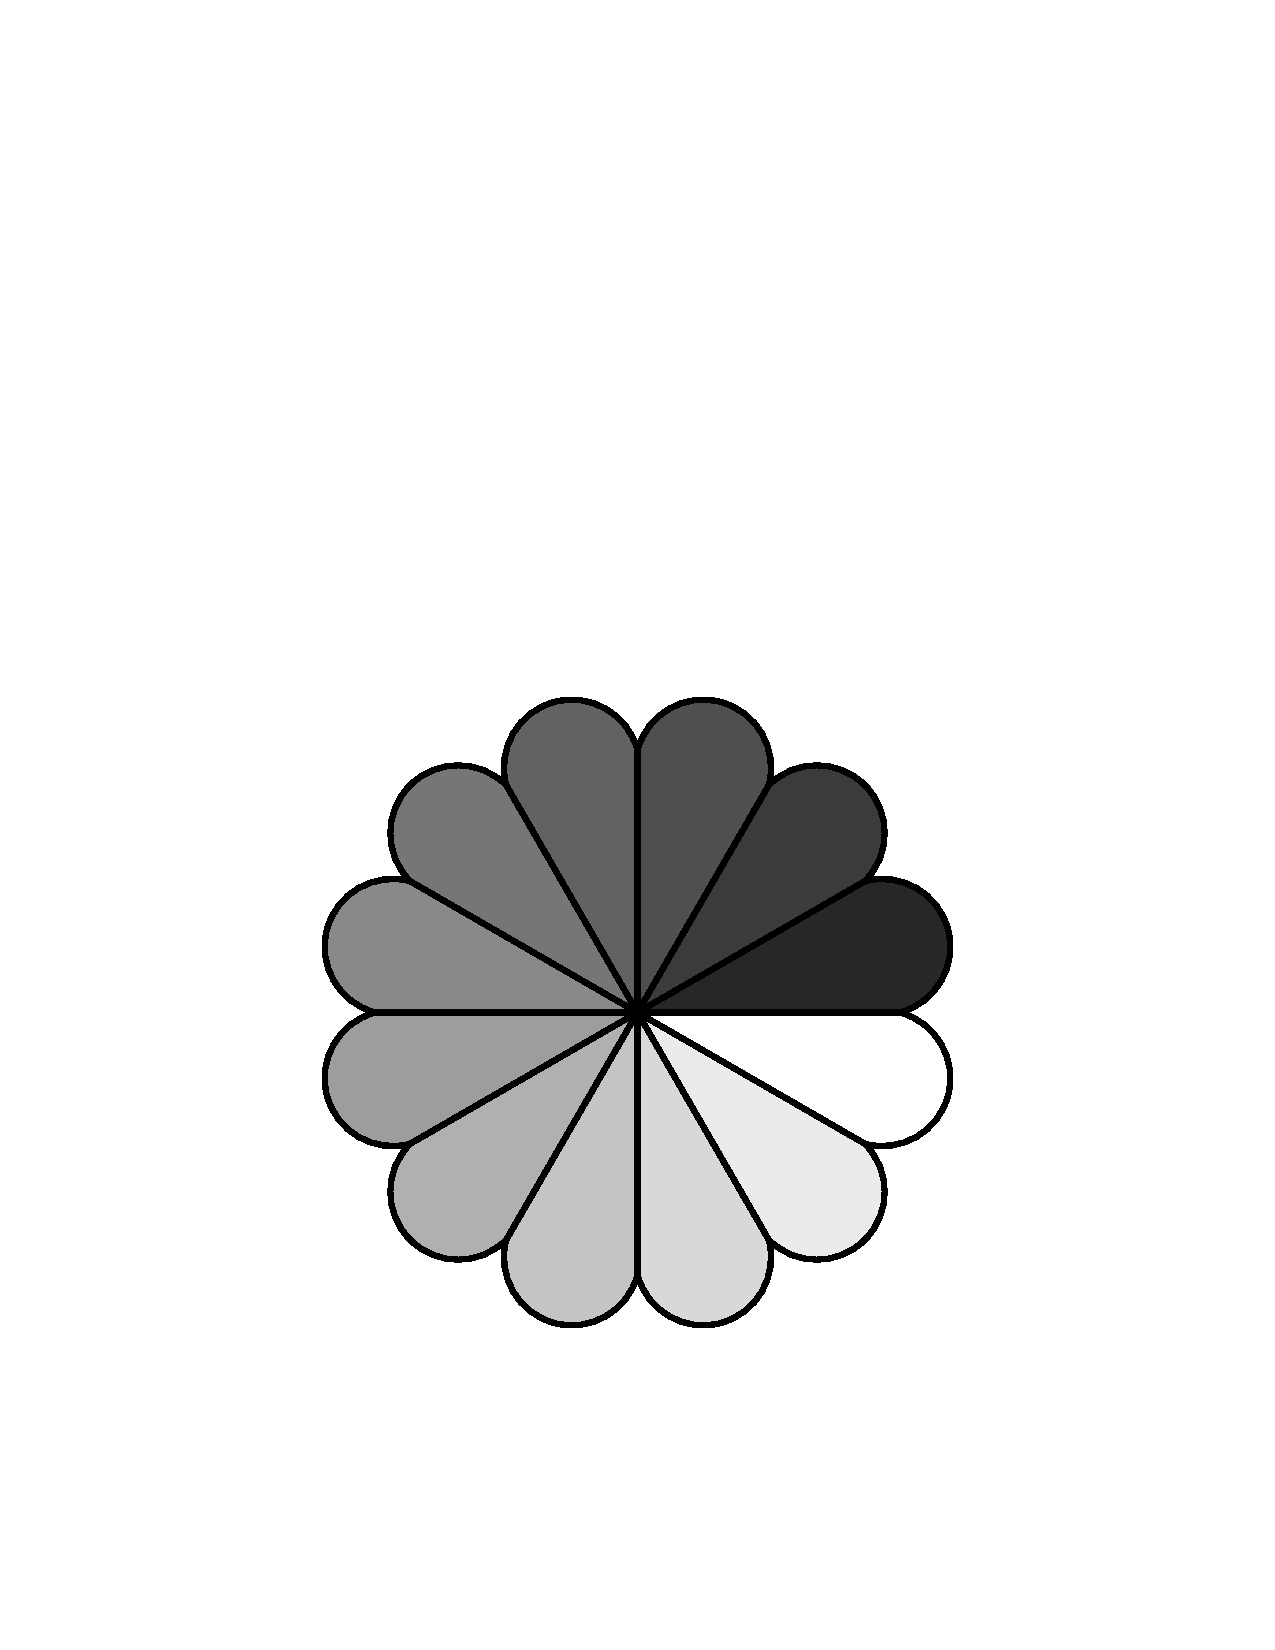
\includegraphics[height=1in,width=1in]{rosette}
\caption{A sample black and white graphic (.pdf format) that has
been resized with the \texttt{includegraphics} command.}
\vskip -6pt
\end{figure}

\subsection{Theorem-like Constructs}
Other common constructs that may occur in your article are
the forms for logical constructs like theorems, axioms,
corollaries, and proofs.  There are
two forms, one produced by the
command \texttt{{\char'134}newtheorem} and the
other by the command \texttt{{\char'134}newdef}; perhaps
the clearest and easiest way to distinguish them is
to compare the two in the output of this sample document:

This uses the \textbf{theorem} environment, created by
the\linebreak\texttt{{\char'134}newtheorem} command:
\newtheorem{theorem}{Theorem}
\begin{theorem}
Let $f$ be continuous on $[a,b]$.  If $G$ is
an antiderivative for $f$ on $[a,b]$, then
\begin{displaymath}\int^b_af(t)dt = G(b) - G(a).\end{displaymath}
\end{theorem}

The other uses the \textbf{definition} environment, created
by the \texttt{{\char'134}newdef} command:
\newdef{definition}{Definition}
\begin{definition}
If $z$ is irrational, then by $e^z$ we mean the
unique number which has
logarithm $z$: \begin{displaymath}{\log e^z = z}\end{displaymath}
\end{definition}

Two lists of constructs that use one of these
forms is given in the
\textit{Author's  Guide}.
 
There is one other similar construct environment, which is
already set up
for you; i.e., you must \textit{not} use
a \texttt{{\char'134}newdef} command to
create it: the \textbf{proof} environment.  Here
is an example of its use:
\begin{proof}
Suppose on the contrary there exists a real number $L$ such that
\begin{displaymath}
\lim_{x\rightarrow\infty} \frac{f(x)}{g(x)} = L.
\end{displaymath}
Then
\begin{displaymath}
l=\lim_{x\rightarrow c} f(x)
= \lim_{x\rightarrow c}
\left[ g{x} \cdot \frac{f(x)}{g(x)} \right ]
= \lim_{x\rightarrow c} g(x) \cdot \lim_{x\rightarrow c}
\frac{f(x)}{g(x)} = 0\cdot L = 0,
\end{displaymath}
which contradicts our assumption that $l\neq 0$.
\end{proof}

Complete rules about using these environments and using the
two different creation commands are in the
\textit{Author's Guide}; please consult it for more
detailed instructions.  If you need to use another construct,
not listed therein, which you want to have the same
formatting as the Theorem
or the Definition \cite{salas:calculus} shown above,
use the \texttt{{\char'134}newtheorem} or the
\texttt{{\char'134}newdef} command,
respectively, to create it.

\subsection*{A {\secit Caveat} for the \TeX\ Expert}
Because you have just been given permission to
use the \texttt{{\char'134}newdef} command to create a
new form, you might think you can
use \TeX's \texttt{{\char'134}def} to create a
new command: \textit{Please refrain from doing this!}
Remember that your \LaTeX\ source code is primarily intended
to create camera-ready copy, but may be converted
to other forms -- e.g., HTML. If you inadvertently omit
some or all of the \texttt{{\char'134}def}s, recompilation will
be, to say the least, problematic.

\begin{figure}
\begin{center}
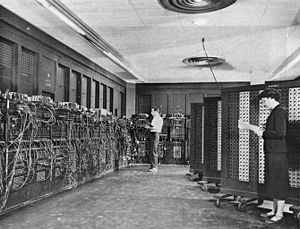
\includegraphics[width=.9\columnwidth]{300px-Eniac.jpg}
\end{center}
\caption{Photograph of Glen Beck (background) and Betty Snyder
  (foreground) programming the ENIAC in BRL building 328. (U.S. Army
  photo), downloaded from wikipedia. This photo was automatically
  resized to ${\frac{9}{10}}$ of the text column using
  the \textbf{includegraphics} command.}
\end{figure}

\section{ASIDE}
I copy/pasted the aside section fomr our recent vlhcc paper for reference. I have added some additional content to make it fit


In this section we describe our prototype interactive static analysis tool, named ASIDE. This version of ASIDE supports both interactive annotation and interactive static analysis. The Interactive annotation takes as input: (a) Abstract Syntax Trees (ASTs) of the application generated by Eclipse JDT or PDT, and (b) a set of security sensitive operations such as operations that read or modify sensitive databases. ASIDE then uses these to generate requests within the IDE for the developer to annotate security related decisions, see Figure~\ref{fig:annotationRequest}. This request is indicated by a yellow highlight of the sensitive code, and a yellow question mark alongside the code. We chose a question mark to try and convey that the tool is requesting information, not indicating anything wrong with the code. Thus, in the example in Figure~\ref{fig:annotationRequest}, the developer was asked to indicate where access control checks are located for the function \textit{updateAccount} that accesses sensitive database tables. Clicking on the icon or code provides a menu where the developer can access ASIDE explanations, as well as choose to enter annotation mode. 

In annotation mode, the developer would then highlight the statements performing access control for the sensitive operation, highlighted in green in Figure~\ref{fig:completedRequest}. In doing so, the developer is reminded to add such checks, if they are not already implemented. ASIDE indicates the annotation with a green highlight and a small green diamond next to the code. The sensitive operation also turns green when an annotation is added, with the icon changing to a green check mark. Even when there are no vulnerabilities detected and no further interaction required by ASIDE, we choose to keep the green icons visible to allow developers to further modify annotations and interact with ASIDE as they continue development. Once the annotation is made, ASIDE leaves annotation mode and the developer returns to the task of coding. 

With the annotations provided by the developer, static analysis is used to detect vulnerabilities. This currently utilizes a path coverage algorithm, which analyzes all paths from the web entry point of the code to the security sensitive operation, ensuring that all paths go through the annotated security checks. Paths without all of the checks are flagged as potential vulnerabilities, and presented as warnings to the developer.  Alternatively, repeated sensitive operations are detected, such as other calls to the function \textit{updateAccount}, and differing access control logic is flagged as a potential vulnerability. In other words, our tool utilizes a standard static analysis technique that assumes that the same operations should be protected by the same access control logic. If the annotated access control logic differs between multiple instances of the same operation, all of those instances are flagged as containing a potential vulnerability. Due to space constraints, we cannot provide all the details of how our path coverage and vulnerability detection algorithm work, but it is fully explained in our recent publication \cite{sacmat2015}.  

A vulnerability warning would be presented as shown in Figure~\ref{fig:warning}, with the red highlighted code and red flag icon. Clicking on the warning would again provide a menu of options, brief explanations of the warning (e.g. the access control logic and the other operations that are related to this warning), and access to more detailed help regarding access control vulnerabilities. Developers can fix the warning by changing the code, and re-annotating the correct access control. Alternatively, they can dismiss the warning if they decide there is not a vulnerability.

This stuff is new. I think we should talk about the input validation part here. We should mention the contextualized stuff

This version of ASIDE also supports warnings involving improper input validation. As developers type, static analysis is carried out behind the scenes. When issues are detected, developers are shown warnings similar to a colored icon on the left margin of the code editing window. These warnings are also accompanied by highlighted text. Developers can then click on these icons and view a contextualized description of why the warning is there (change wording later). Developers can then choose from a variety of quick fixes, as shown in figure (add this later). These quick fixes then auto generate code to solve the issue. One of these quickfixes, called "Read More" opens a webpage which contains much more contextualied help for the specific issue. For sql injection warnings, autogenerated code options were not provided, since prepared statements should be used to solve the problem.


\begin{figure}[h]
\centering
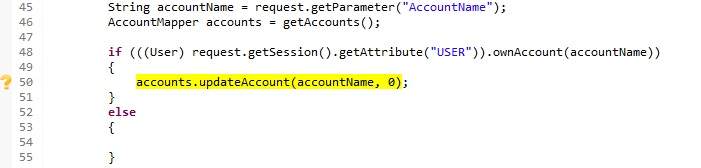
\includegraphics[width=0.5\textwidth]{annotationRequest}
\caption{Annotation request in Gold Rush, shown with a yellow highlight and question mark icon.}
\label{fig:annotationRequest}
\end{figure}

\begin{figure}[h]
\centering
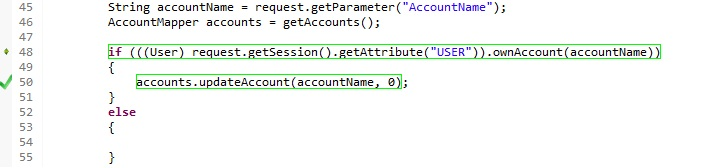
\includegraphics[width=0.5\textwidth]{completedRequest}
\caption{An annotation and annotation request that have been completed in Gold Rush. The completed request is shown with a green highlight and green checkmark icon.}
\label{fig:completedRequest}
\end{figure}

\begin{figure}
\centering
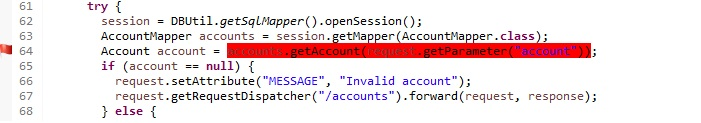
\includegraphics[width=0.5\textwidth]{warning}
\caption{ASIDE example with sample code in Gold Rush. A warning is displayed on line 64}
\label{fig:warning}
\end{figure}



\section{Methodology}
We designed a user study to examine user interaction with the contextualized version of our interactive static analysis and interactive annotation prototype. First we wanted to assess how intuitive our interface is for developers. Second, we wished to understand developer's perceptions of our combined prototype. Third, we wanted to assess the effectiveness of our tool in assisting developers with understanding potential security vulnerabilities regarding sql injection, cross site scripting, and access control.

We recruited actual professional developers from various companies to conduct our study. There job titles included the following: (list all job titles).  They had an average of X years of experience as professional Java Developers. To recruit these developers, we used a snowball sample. We asked developers we knew, and we asked them to recommend additional participants. To compensate developers for their time, we awarded a  \$25 gift card to each participant.

Participants interacted with ASIDE running on a project called Gold Rush, an internally developed Java-based banking application (99 files) to teach web application security. When participants were interested, we would send them an email with a consent form. Participants would then individually book a time to perform the study and reply back saying they consent. At the booked time, they would call us from a remote location, and login to our computer through the use of remote desktop software. Participants were then given a brief introduction to ASIDE. They were then shown and allowed to interact with a trainer example, which consisted of one input validation warning. The purpose of the example was to answer any questions they had before beginning and to account for Eclipse interface quirks which could not be removed or fixed in our current prototype.

We would then show the participant a serious of warnings and ask participants which option they would choose. Afterwards, we would ask them a set of questions, which were the same for all of the warnings. If they did not visit the ``Read More'' pages, we would prompt them to do so when they had examined all of the warnings. Once they had observed all of the warnings, we showed them a very brief example of an annotation request and an annotation. During the demonstration, the researcher would perform an annotation. Then, the participant was asked to create annotations for two annotation requests. After each of these, we asked several questions. The questions were the same for each of the annotation requests. Once this was done, we asked several questions about aside as a whole and asked them to provide answers for a demographic survey. Throughout the study, participants were shown the same warnings and annotation requests, in the same order. Call recording and screen recording software were used to capture the activities of the participant on screen and the responses. The primary author performed open coding on the transcriptions and notes, to determine performance and look for common patterns and interesting responses


\section{Results}
These are some of our findings from examining the data. We will flesh them out, and in more detail, and eventually have a results section

On the whole, participants seemed to prefer the way ASIDE presented vulnerabilities to the annotation requests. Reason, similar to other tools? Harder? Presented at the end? No access control vulnerability explanation? Emphasis on these types of issues?. Some of them seemed to not understand the reasoning behind the annotations. Perhaps more training (like the last study) is needed. They also were not familar with the code, like the studetns in the previous study were.

Participants wanted quick fixes for everything. They suggested at ways to do it for sql injection and expressed a desire to have it for access control issues.

In terms of the quick fix options, participants hinted at a trade-off between specificity and generality. Particpants did not like "letters and numbers" for cases when only letters or only numbers was ideal. They wanted specific options that fit the specific issue.
 
While addressing the vulnerabilities, some participants griped that ASIDE didn't provide enough background information. Most of them did not attempt to open the contextualized help pages. However, when they found it or were shown it, they were almost always very very pleased to see it. Many suggested that they did not see it because it looked like another quick fix. Also, they didn't realize double clicking it would open a web page. They suggested a link in the descriptions of the other fixes would be better.

Participants were very good at choosing the right options for quick fixes. They moved a lot slower than the students from the previous annotation study, perhaps trying to be more careful. When they understood the annotation approach, they liked it, were skilled at it, and rated it well. Overall, particpants gave very favorable evaluations for the tool. Many likert scale questions were used and we expect those numbers to be favorable.
 
 

\section{Conclusions}
This paragraph will end the body of this sample document.
Remember that you might still have Acknowledgments or
Appendices; brief samples of these
follow.  There is still the Bibliography to deal with; and
we will make a disclaimer about that here: with the exception
of the reference to the \LaTeX\ book, the citations in
this paper are to articles which have nothing to
do with the present subject and are used as
examples only.
%\end{document}  % This is where a 'short' article might terminate

%ACKNOWLEDGMENTS are optional
\section{Acknowledgments}
This section is optional; it is a location for you
to acknowledge grants, funding, editing assistance and
what have you.  In the present case, for example, the
authors would like to thank Gerald Murray of ACM for
his help in codifying this \textit{Author's Guide}
and the \textbf{.cls} and \textbf{.tex} files that it describes.

%
% The following two commands are all you need in the
% initial runs of your .tex file to
% produce the bibliography for the citations in your paper.
\bibliographystyle{abbrv}
\bibliography{sigproc}  % sigproc.bib is the name of the Bibliography in this case
% You must have a proper ".bib" file
%  and remember to run:
% latex bibtex latex latex
% to resolve all references
%
% ACM needs 'a single self-contained file'!
%
%APPENDICES are optional
%\balancecolumns
\appendix
%Appendix A
\section{Headings in Appendices}
The rules about hierarchical headings discussed above for
the body of the article are different in the appendices.
In the \textbf{appendix} environment, the command
\textbf{section} is used to
indicate the start of each Appendix, with alphabetic order
designation (i.e., the first is A, the second B, etc.) and
a title (if you include one).  So, if you need
hierarchical structure
\textit{within} an Appendix, start with \textbf{subsection} as the
highest level. Here is an outline of the body of this
document in Appendix-appropriate form:
\subsection{Introduction}
\subsection{The Body of the Paper}
\subsubsection{Type Changes and  Special Characters}
\subsubsection{Math Equations}
\paragraph{Inline (In-text) Equations}
\paragraph{Display Equations}
\subsubsection{Citations}
\subsubsection{Tables}
\subsubsection{Figures}
\subsubsection{Theorem-like Constructs}
\subsubsection*{A Caveat for the \TeX\ Expert}
\subsection{Conclusions}
\subsection{Acknowledgments}
\subsection{Additional Authors}
This section is inserted by \LaTeX; you do not insert it.
You just add the names and information in the
\texttt{{\char'134}additionalauthors} command at the start
of the document.
\subsection{References}
Generated by bibtex from your .bib file. Run latex,
then bibtex, then latex twice (to resolve references)
to create the .bbl file. Insert that .bbl file into
the .tex source file and comment out
the command \texttt{{\char'134}thebibliography}.
% This next section command marks the start of
% Appendix B, and does not continue the present hierarchy
\section{More Help for the Hardy}
The sig-alternate.cls file itself is chock-full of succinct
and helpful comments. If you consider yourself a moderately
experienced to expert user of \LaTeX, you may find reading
it useful but please remember not to change it.
%\balancecolumns % GM June 2007
% That's all folks!
\end{document}
